\documentclass[german]{../spicker}

\usepackage{amsmath}
\usepackage{polynom}
\usepackage{array}   % for \newcolumntype macro
\usepackage{tikz}
\usepackage{pgfplots}
\usepgfplotslibrary{fillbetween}
\pgfplotsset{compat=1.17}
\title{Analysis 1}
\author{Patrick Gustav Blaneck, Felix Racz}
\makeindex[intoc]
\makeindex[intoc, name=Beispiele,title=Beispiele]

\newcommand{\scalarprod}[1]{\left\langle #1 \right\rangle}
\newcommand{\vektor}[1]{\begin{pmatrix*}[r] #1 \end{pmatrix*}}
\renewcommand{\span}[1]{\operatorname{span}\left(#1\right)}

\renewcommand{\abs}[1]{\left| #1 \right|}
\newcommand{\cis}[1]{\left( \cos\left( #1 \right) + i \sin\left( #1 \right) \right)}
\newcommand{\sgn}{\text{sgn}}
\newcommand{\diff}{\mathrm{d}}
\newcommand{\dx}{~\mathrm{d}x}
\newcommand{\du}{~\mathrm{d}u}
\newcommand{\dv}{~\mathrm{d}v}
\newcommand{\dw}{~\mathrm{d}w}
\newcommand{\dt}{~\mathrm{d}t}
\newcommand{\dn}{~\mathrm{d}n}
\newcommand{\dudx}{~\frac{\mathrm{d}u}{\mathrm{d}x}}
\newcommand{\dudn}{~\frac{\mathrm{d}u}{\mathrm{d}n}}
\newcommand{\dvdx}{~\frac{\mathrm{d}v}{\mathrm{d}x}}
\newcommand{\dwdx}{~\frac{\mathrm{d}w}{\mathrm{d}x}}
\newcommand{\dtdx}{~\frac{\mathrm{d}t}{\mathrm{d}x}}
\newcommand{\ddx}{\frac{\mathrm{d}}{\mathrm{d}x}}
\newcommand{\dFdx}{\frac{\mathrm{d}F}{\mathrm{d}x}}
\newcommand{\dfdx}{\frac{\mathrm{d}f}{\mathrm{d}x}}
\newcommand{\interval}[1]{\left[ #1 \right]}

\newcolumntype{L}{>{$}l<{$}} % math-mode version of "l" column type
\newcolumntype{R}{>{$}r<{$}} % math-mode version of "r" column type
\newcolumntype{C}{>{$}c<{$}} % math-mode version of "c" column type
\newcolumntype{P}{>{$}p<{$}} % math-mode version of "l" column type

\begin{document}
\maketitle
\tableofcontents
\newpage

%\setcounter{section}{1}

\section{Grundlagen}

\subsection{Funktionen}

\begin{thirdboxl}
    \begin{defi}{Injektivität}
        $f(x) = f(x')\implies x = x'$
    \end{defi}
\end{thirdboxl}%
\begin{thirdboxm}
    \begin{defi}{Surjektivität}
        $\forall y, \exists x: y = f(x)$
    \end{defi}
\end{thirdboxm}%
\begin{thirdboxr}
    \begin{defi}{Bijektivität}
        $\forall y, \exists! x: y = f(x)$
    \end{defi}
\end{thirdboxr}%

\begin{algo}{Beweisen der Injektivität}
    \begin{enumerate}
        \item Behauptung: $f(x) = f(x')$
        \item Umformen auf eine Aussage der Form $x = x'$
    \end{enumerate}
\end{algo}

\begin{algo}{Beweisen der Surjektivität}
    \begin{enumerate}
        \item Aufstellen der Umkehrfunktion
        \item Zeigen, dass diese Umkehrfunktion auf dem gesamten Definitionsbereich definiert ist
    \end{enumerate}
\end{algo}

\begin{algo}{Beweisen der Bijektivität}
    \begin{enumerate}
        \item Injektivität beweisen
        \item Surjektivität beweisen
    \end{enumerate}
\end{algo}

\subsection{Polynome}

\begin{defi}{Polynom}
    Eine Funktion $p(x) = \sum^n_{i=0} a_i x^i$ mit $a_i, x \in \R ~ (\C), a_n \neq 0$ heißt \emph{Polynom vom Grad} $n$.
\end{defi}

\begin{halfboxl}
    \vspace{-\baselineskip}
    \begin{bonus}{Abspalten von Linearfaktoren}
        Sei $x_0$ eine Nullstelle eines Polynoms $p(x)$, dann ist
        $$ p(x) = q(x) \cdot (x-x_0).$$
        Dabei ist $(x-x_0)$ ein abgespaltener Linearfaktor und $q(n)$ das entsprechend reduzierte Polynom mit $q(n) = \frac{p(x)}{x-x_0}$.
    \end{bonus}
\end{halfboxl}%
\begin{halfboxr}
    \vspace{-\baselineskip}
    \begin{bonus}{Faktorisierung}
        Sind $x_1, \ldots, x_n$ Nullstellen eines Polynoms $p(x)$, so ist
        $$ p(x) = a_n \cdot (x-x_1) \cdot \ldots \cdot (x-x_n)$$
        die Faktorisierung von $p(x)$.
    \end{bonus}
\end{halfboxr}%

\subsubsection*{Polynome vom Grad 2}
\begin{halfboxl}
    \vspace{-\baselineskip}
    \begin{algo}{$pq$-Formel}
        \begin{enumerate}
            \item Polynom der Form $x^2 + px + q = 0$
            \item $x_{1,2} = -\frac{p}{2} \pm \sqrt{\left(\frac{p}{2}\right)^2 - q}$
        \end{enumerate}
    \end{algo}
\end{halfboxl}%
\begin{halfboxr}
    \vspace{-\baselineskip}
    \begin{algo}{Mitternachtsformel}
        \begin{enumerate}
            \item Polynom der Form $ax^2 + bx + c = 0$
            \item $x_{1,2} = \frac{-b \pm \sqrt{b^2 - 4ac}}{2a}$
        \end{enumerate}
    \end{algo}
\end{halfboxr}

\begin{bonus}{Besonderheiten bei $x \in \C$}
    \begin{itemize}
        \item Ist $x_i$ eine Nullstelle des Polynoms $p(x)$ mit \emph{reellen Koeffizienten}, dann ist auch $\overline{x_i}$ eine Nullstelle von $p(x)$.
    \end{itemize}
\end{bonus}

\subsection{Gebrochen rationale Funktionen}

\begin{defi}{Gebrochen rationale Funktionen}
    Seien $p_m(x)$ und $p_n(x)$ Polynome vom Grad $m$ bzw. $n$, dann heißt
    $$
        f(x) = \frac{p_m(x)}{p_n(x)}
    $$
    \emph{gebrochen rationale Funktion}.\\
    Im Fall $m<n$ heißt die Funktion \emph{echt gebrochen rational}, sonst \emph{unecht gebrochen rational}.
\end{defi}

\begin{algo}{Polynomdivision}
    Gegeben ist \emph{unecht gebrochen rationale Funktion} $f(x) = \frac{p_m(x)}{p_n(x)}$
    \begin{enumerate}
        \item \emph{Dividiere} die größten Exponenten aus beiden Polynomen
        \item \emph{Mutipliziere} Ergebnis mit Divisor zurück
        \item \emph{Subtrahiere} Ergebnis vom Dividenden
        \item Wiederhole, bis:
              \subitem Ergebnis 0 ist, oder
              \subitem Grad des Ergebnisses kleiner ist als Grad des Divisors (ergibt \emph{Rest})
    \end{enumerate}
\end{algo}

%\begin{bonus}{Polynomdivision Beispiel}
%    \polylongdiv[style=C]{x^3+x^2-1}{x-1}
%\end{bonus}

\begin{algo}{Hornerschema}
    Gegeben ist \emph{Polynom} $p_m(x)$ und ein \emph{Wert} $x_0$

    Vorbereitung:
    \begin{itemize}
        \item Erstelle eine Tabelle mit $m + 2$ Spalten und 3 Zeilen
        \item Erste Zelle frei lassen und dann Koeffizienten $a_m, a_{m-1}, \ldots, a_0$ in die erste Zeile schreiben
        \item In die erste Zelle der zweiten Zeile kommt $x_0$
    \end{itemize}

    Anwendung (beginnend in zweiter Zelle der dritten Zeile):
    \begin{enumerate}
        \item Erster Koeffizient der ersten Zeile in die dritte Zeile
        \item \emph{Multipliziere} Zahl der ersten Spalte mit diesem Koeffizienten
        \item Schreibe Ergebnis in zweite Zeile, unterhalb des nächsten Koeffizienten
        \item \emph{Addiere} Ergebnis mit diesem Koeffizienten
        \item Wiederhole 2-4 bis zum Schluss
    \end{enumerate}

    Ergebnis:
    \begin{itemize}
        \item Wert des Polynoms $p_m(x_0)$ in letzter Zelle der letzten Zeile
        \item Bei Wert $p_m(x_0) = 0$ steht in der letzten Zeile das Polynom nach Abspalten des Linearfaktors $(x-x_0)$
    \end{itemize}
\end{algo}

%\begin{bonus}{Hornerschema Beispiel}
%    Gegeben: $p_4(x) = 2x^4-3x^3+4x^2-5x+2$ an der Stelle $x_0 = 1$
%    \polyhornerscheme[x=1]{2x^4-3x^3+4x^2-5x+2}
%    Ergebnis: $p_4(1) = 0 \implies (x-1) \text{ ist Linearfaktor von } p_4(x) \text{ und } \frac{p_4(x)}{x-1} = 2x^3 = x^2 + 3x -2$
%\end{bonus}

\begin{bonus}{Tipps und Tricks}
    \begin{itemize}
        \item Polynomdivision und Hornerschema funktionieren auch sehr gut mit komplexen Zahlen
        \item Bei mehreren abzuspaltenden Linearfaktoren bietet sich das Hornerschema sehr gut an
    \end{itemize}
\end{bonus}

\begin{algo}{Partialbruchzerlegung}
    Gegeben: \emph{Echt gebrochen rationale Funktion}  $f(x) = \frac{p_m(x)}{p_n(x)}$
    \begin{enumerate}
        \item Berechne Nullstellen des \emph{Nennerpolynoms} $x_0, \ldots, x_k \in \R$
        \item Verschiedene Fälle:
              \subitem Relle Nullstellen:
              \subsubitem $x_i$ ist einfache Nullstelle $\implies \frac{A}{x-x_1}$
              \subsubitem $x_i$ ist $r$-fache Nullstelle $\implies  \frac{A_1}{x-x_1} +  \frac{A_2}{(x-x_1)^2} + \ldots + \frac{A_r}{(x-x_1)^r}$
              \subitem Nichtrelle Nullstellen:
              \subsubitem Einfacher quadratischer Term $\implies \frac{Ax + B}{x^2+px+q}$
              \subsubitem $r$-facher quadratischer Term $\implies \frac{A_1x + B_1}{x^2+px+q} + \frac{A_2x + B_2}{(x^2+px+q)^2} + \ldots + \frac{A_rx + B_r}{(x^2+px+q)^r}$
        \item Koeffizientenvergleich:
              \begin{enumerate}
                  \item Brüche gleichnamig machen (Multipliziere beide Seiten mit Nennerpolynom)
                  \item Potenzen von $x$ zusammenfassen
                  \item Gleichungssystem lösen
                  \item Lösungen in Ansatz einsetzen
              \end{enumerate}
    \end{enumerate}
\end{algo}

\begin{bonus}{Besonderheiten in $\C$}
    \begin{itemize}
        \item Für Partialbrüche ohne relle Nullstellen können wir in $\C$ stets Nullstellen finden. Das Verfahren erfolgt dann analog mit komplexen Nullstellen.
    \end{itemize}
\end{bonus}

\begin{bonus}{Tipps und Tricks}
    \begin{itemize}
        \item Partialbruchzerlegung ist erst bei einer \emph{echt gebrochen rationale Funktion} sinnvoll
        \item Ist die Funktion unecht gebrochen rational, führe zuerst eine Polynomdivision durch und zerlege dann den Rest in die Partialbrüche
    \end{itemize}
\end{bonus}


\subsection{Gleichungen und Ungleichungen}

\begin{algo}{Berechnen einer Lösungsmenge bei Ungleichungen}
    Gegeben: Ungleichung mit Bezug auf Variable $x$
    \begin{enumerate}
        \item Für jeden Betrag $\left| a(x) \right|$, eine Fallunterscheidung machen für
              \subitem $a(x) \geq 0 \implies \left| a(x) \right| = a(x)$
              \subitem $a(x) < 0 \implies \left| a(x) \right| = -a(x)$
              \subitem \emph{Hier haben wir bereits eine Einschränkung für die Lösungsmenge des jeweiligen Falles gegeben!}
        \item Ungleichungen nach $x$ auflösen
        \item Jeder Fall $i$ erzeugt eine Lösungsmenge $L_i$ bestehend aus\emph{ umgestellter Ungleichung} und Fallbedingungen
        \item Lösungsmenge $L = \bigcup^n_{i = 1} L_i$, wobei $n$ die Anzahl der betrachteten Fälle ist
    \end{enumerate}
\end{algo}

\begin{bonus}{Tipps und Tricks}
    \begin{itemize}
        \item $n$ Beträge in der Gleichung können zu $2^n$ Fällen führen.
        \item Es kann vorkommen, dass ein Fall einer Fallunterscheidung unerreichbar ist, z.B. für $x > 5 \land x < 1$. Die Lösungsmenge $L$ ist dann leer ($L = \emptyset$).
        \item Radizieren (Wurzelziehen) ist in Ungleichungen nur erlaubt, wenn danach der \emph{Betrag} der Wurzel betrachtet wird
        \item Quadrieren einer Ungleichung `erzeugt' potentiell ein falsches Ergebnis. Nach dem Quadrieren sollte man also jedes Ergebnis prüfen.
        \item Multiplikation mit negativen Zahlen sollte vermieden werden, da das Umdrehen des Ungleichheitszeichens schnell für Flüchtigkeitsfehler sorgen kann.
    \end{itemize}
\end{bonus}

\subsection{Komplexe Analysis}
\begin{bonus}{Rechenregeln für komplexe Zahlen in kartesischen Koordinaten}
    \textbf{Darstellung:} $z = a + i \cdot b$ und $w = c + i \cdot d$

    \textbf{Addition und Subtraktion:} $z \pm w = (a\pm c) + i \cdot (b \pm d)$

    \textbf{Multiplikation:} $z \cdot w = (ac -bd) + i \cdot (ad + bc)$

    \textbf{Division:} $\frac{z}{w} = \frac{z \cdot \overline{w}}{w \cdot \overline{w}}$

    \textbf{Komplex konjugiert:} Vorzeichen von $\Im$ wechseln: $\overline{z} = a- i \cdot b$

    \textbf{Betrag:} Abstand vom Ursprung: $\abs{z} = \sqrt{z \cdot \overline{z}} = \sqrt{a^2 + b^2}$
\end{bonus}

\begin{bonus}{Rechenregeln für komplexe Zahlen in Polarkoordinaten}
    \textbf{Darstellung:} $z = r \cdot (\cos\theta + i \cdot \sin \theta) = r \cdot e^{i \cdot \theta}$

    \textbf{Multiplikation:} $z \cdot w = r_z \cdot r_w \cdot e^{i \cdot (\theta_z + \theta_w)}$

    \textbf{Division:} $\frac{z}{w} = \frac{r_z}{r_w} \cdot e^{i \cdot (\theta_z - \theta_w)}$

    \textbf{Komplex konjugiert:} $\overline{z} = (r, -\theta) = (r, 2\pi - \theta)$

    \textbf{Betrag:} $\abs{z} = r$
\end{bonus}

\begin{algo}{Kartesische Koordinaten $\to$ Polarkoordinaten}
    \begin{enumerate}
        \item $r = \abs{z} = \sqrt{x^2 + y^2}$
        \item
              \subitem $y \geq 0 : \theta = \arctan \frac{x}{r}$
              \subitem $y < 0 : \theta = -\arctan \frac{x}{r}$
    \end{enumerate}
\end{algo}

\begin{algo}{Polarkoordinaten $\to$ Kartesische Koordinaten}
    \begin{enumerate}
        \item $x = r \cdot \cos \theta$
        \item $y = r \cdot \sin \theta$
    \end{enumerate}
\end{algo}

\begin{algo}{Radizieren von komplexen Zahlen}
    Gesucht: Lösung von $z^n = r \cdot e^{i\cdot \theta}$
    \begin{enumerate}
        \item Ist $z^n$ nicht in Polarkoordinaten gegeben, so ist zunächst die Polarform zu bilden.
        \item Bertechne $r_k = \sqrt[n]{r}$. Dieser Radius ist die Länge aller Lösungen.
        \item Berechne für alle $k \in [0, n-1]$
              $$
                  \theta_k = \frac{\theta + k\cdot 2\pi}{n} = \frac{\theta}{n} + \frac{k}{n} \cdot 2\pi
              $$
        \item Die Lösungen sind dann die $n$ Zahlen $z_k = (r_k, \theta_k)$ für $k \in [0, n-1]$.
    \end{enumerate}
    \qed
\end{algo}

\section{Folgen und Reihen}

\subsection{Grundlagen}
\begin{bonus}{Rechenregeln für Summen}
    $$
        \begin{aligned}
            \sum_{k=m}^n a_k                    & = \sum_{k=m-l}^{n-l} a_{k+l}          \\
            \sum_{k=m}^n a_k                    & = \sum_{k=m}^c a_k + \sum_{k=c}^n a_k \\
            \sum_{k=m}^n a_k + \sum_{k=m}^n b_k & = \sum_{k=m}^n a_k + b_k              \\
            \sum_{k=m}^n c\cdot a_k             & = c\cdot\sum_{k=m}^n a_k
        \end{aligned}
    $$
    Die Regeln gelten auch für unendliche Reihen.
\end{bonus}

\begin{bonus}{Wichtige Summen}
    \begin{itemize}
        \item Arithmetische Summe: $$\sum^n_{k=1} k = \frac{n(n+1)}{2}$$
        \item Geometrische Summe: $$\sum^n_{k=1} x^k = \frac{1-x^{n+1}}{1-x} = \frac{x^{n+1} - 1}{x-1}$$
        \item Summe der Quadratzahlen: $$\sum^n_{k=1} k^2 = \frac{n(n+1)(2n+1)}{6}$$
        \item Summe der Kubikzahlen: $$\sum^n_{k=1} k^3 = \left(\frac{n(n+1)}{2}\right)^2$$
    \end{itemize}
\end{bonus}

\subsection{Binomialkoeffizienten und der binomische Lehrsatz}

\begin{defi}{Binomialkoeffizient}
    Die Anzahl der $k$-elementigen Teilmengen einer $n$-elementigen Menge bezeichnen wir mit $\binom{n}{k}$.
    Diese Zahlen heißen \emph{Binomialkoeffizienten} oder Binomialzahlen.
\end{defi}

\begin{defi}{Rekursionsformel für Binomialkoeffizient}
    Für $k, n \in \N$ mit $k \leq n$ gilt:
    $$
        \binom{n}{k} = \binom{n-1}{k} + \binom{n-1}{k-1}
    $$
\end{defi}

\begin{defi}{Kombinatorische Formel für Binomialkoeffizient}
    $$
        \binom{n}{k} = \begin{cases}
            0                          & , \text{ für } k > n    \\
            \frac{n!}{(n-k)! \cdot k!} & , \text{ für } k \leq n
        \end{cases}
    $$
\end{defi}

\begin{defi}{Der binomische Lehrsatz}
    Für beliebige $a, b \in \R$ und $n \in \N$ gilt:
    $$
        (a+b)^n = \sum^n_{k=0} \binom{n}{k} a^k \cdot b^{n-k}
    $$
\end{defi}

\section{Konvergenz von Folgen, Reihen und Funktionen}

\subsection{Grundlagen}
\begin{defi}{Schranken}
    Gilt $$\forall x\in A : \abs{x} < K,$$ so heißt die Menge $A$ \emph{beschränkt} und $K$ \emph{Schranke}.

    Gilt nur $x \leq K$, so heißt die Menge \emph{nach oben beschränkt} und $K$ \emph{obere Schranke}.

    Im Falle $x \geq K$ heißt $A$ \emph{nach unten beschränkt} und $K$ \emph{untere Schranke}.
\end{defi}

\begin{defi}{Beschränktheit}
    Eine Menge $M$ heißt genau dann \emph{beschränkt}, wenn sie nach oiben und nach unten beschränkt ist.
\end{defi}

\begin{defi}{Supremum, Maximum}
    Der Wert
    $$
        K= \min_{K^* \in \R} \{K \text{ ist obere Schranke}\}
    $$
    heißt \emph{kleinste obere Schranke} oder \emph{Supremum von A}.
    Notation: $\sup A$

    Gilt $K \in A$, so heißt $K$ \emph{Maximum von A}. Notation: $\max A$.
\end{defi}

\begin{defi}{Infimum, Minimum}
    Der Wert
    $$
        K= \max_{K^* \in \R} \{K \text{ ist untere Schranke}\}
    $$
    heißt \emph{größte untere Schranke} oder \emph{Infimum von A}.
    Notation: $\inf A$

    Gilt $K \in A$, so heißt $K$ \emph{Minimum von A}. Notation: $\min A$.
\end{defi}

\begin{bonus}{Vollständigkeitsaxiom}
    Jede nicht-leere nach oben beschränkte Menge $A$ hat ein \emph{Supremum}, jede nicht-leere nach unten beschränkte Menge $A$ hat ein \emph{Infimum}.
\end{bonus}

\begin{defi}{$\epsilon$-Umgebung von $K$ in $\R$}
    $$
        U_\epsilon(K) := \{ x \in \R \mid \abs{x - K} < \epsilon \}
    $$
    heißt $\epsilon$\emph{-Umgebung von} $K$ \emph{in} $\R$.
\end{defi}

\begin{defi}{Innerer Punkt}
    $x_0 \in A$ heißt \emph{innerer Punkt von A}, falls eine $\epsilon$-Umgebung existiert, so dass $U_\epsilon (x_0) \in A$, also vollständig in $A$ enthalten ist.
    $A$ heißt \emph{offen}, falls jeder Punkt der Menge innerer Punkt ist.
\end{defi}

\begin{defi}{Häufungspunkt (Mengen)}
    $a$ heißt \emph{Häufungspunkt einer Menge A}, wenn $\forall \epsilon > 0$ in der Umgebung $U_\epsilon (a)$ ein Punkt $x \in A$ mit $x \neq a$ existiert.

    Sei $x$ größter Häufungspunkt von $A$, dann heißt
    $$
        x = \lim\sup A \text{ (Limes Superior).}
    $$

    Sei $x$ kleinster Häufungspunkt von $A$, dann heißt
    $$
        x = \lim\inf A \text{ (Limes Inferior).}
    $$
\end{defi}

\begin{defi}{Abgeschlossenheit}
    $A$ heißt \emph{abgeschlossen}, wenn jeder Häufungspunkt von $A$ in $A$ liegt.
\end{defi}

\begin{defi}{Bolzano-Weierstrass für Mengen}
    Jede unendliche beschränkte Menge $A$ reeller Zahlen besitzt mindestens einen Häufungspunkt.
\end{defi}

\subsection{Konvergenz von Folgen}

\begin{defi}{Monotonie}
    Eine Folge $a_n$ heißt \emph{monoton wachsend}, falls $\forall n \in \N : a_n \leq a_{n+1}$.
    Gilt sogar $a_n < a_{n+1}$, so heißt die Folge \emph{streng monoton wachsend}.

    Eine Folge $a_n$ heißt \emph{monoton fallend}, falls $\forall n \in \N : a_n \geq a_{n+1}$.
    Gilt sogar $a_n > a_{n+1}$, so heißt die Folge \emph{streng monoton fallend}.
\end{defi}

\begin{defi}{Häufungspunkt (Folgen)}

    $a$ heißt \emph{Häufungspunkt einer Folge}, wenn zu jeder $\epsilon$-Umgebung $U_\epsilon (a)$ unendlich viele Folgenglieder $a_n$ in $U_\epsilon (a)$ liegen, also
    $$
        \forall \epsilon > 0 , \exists \infty\text{-viele } a_n : \abs{a_n - a} < \epsilon
    $$
\end{defi}

\begin{defi}{Grenzwert / Limes}
    Eine Zahl $a\in \R \text{ oder } \C$ heißt \emph{Grenzwert} oder \emph{Limes} einer Zahlenfolge $a_n$, wenn $\forall \epsilon >0, \exists n_0 (\epsilon)$, so dass für alle $n \geq n_0 (\epsilon)$ (fast immer) gilt
    $$
        \abs{a_n - a} < \epsilon
    $$

    Jeder Grenzwert ist auch ein Häufungspunkt.
\end{defi}

\begin{defi}{Konvergenz / Divergenz}
    Eine Folge $a_n$ heißt \emph{konvergent}, falls ein Grenzwert existiert.

    Existiert dieser nicht, so heißt die Folge \emph{divergent}.

    Eine konvergente Folge mit $a=0$ heißt \emph{Nullfolge}.

    Ist $\lim_{n\to\infty}a_n = a$, so ist $\lim_{n\to\infty}(a_n-a) = 0$, d.h. $b_n=\lim_{n\to\infty}(a_n-a)$ ist \emph{Nullfolge}.
\end{defi}

\begin{defi}{Bolzano-Weierstrass für Folgen}
    1. Jede beschränkte Folge $a_n$ besitzt mindestens eine konvergente Teilfolge.

    2. Jede beschränkte Folge $a_n$ besitzt einen kleinsten und größten Häufungspunkt mit $b \geq a$
    $$
        \begin{aligned}
            a & = \lim\inf a_n, \\
            b & = \lim\sup a_n.
        \end{aligned}
    $$
    3. Eine Folge konvergiert genau dann, wenn sie beschränkt ist und nur einen Häufungspunkt besitzt. Dann ist
    $$
        a = \lim_{n\to\infty} a_n = \lim\inf a_n = \lim\sup a_n.
    $$
\end{defi}

\begin{defi}{Sandwich-Lemma oder Einschnürungssatz}
    Gilt fast immer, also bis auf endliche viele $n$ (oder auch für $n \geq n_0$)
    $$
        a_n \leq c_n \leq b_n
    $$
    und $\lim_{n\to\infty}a_n = a = \lim_{n\to\infty}b_n$, so ist
    $$
        \lim_{n\to\infty}c_n = a.
    $$
\end{defi}

\begin{bonus}{Rechenregeln für Grenzwerte}
    $$
        \begin{aligned}
            \lim_{n\to\infty} (a_n + b_n)     & = a+b                                          \\
            \lim_{n\to\infty} c\cdot a_n      & = c \cdot a                                    \\
            \lim_{n\to\infty} a_nb_n          & = a \cdot b                                    \\
            \lim_{n\to\infty} \frac{a_n}{b_n} & = \frac{a}{b} \text{ für } b_n \neq 0, b\neq 0 \\
            \lim_{n\to\infty} \frac{1}{a_n}   & = \frac{1}{a} \text{ für } a_n \neq 0, a\neq 0
        \end{aligned}
    $$
\end{bonus}

\begin{bonus}{Wichtige Grenzwerte}
    $$
        \begin{aligned}
            \lim_{n\to\infty} \frac{1}{n^\alpha} & = 0 \text{ für } \alpha >0             \\
            \lim_{n\to\infty} \sqrt[n]{a}        & = 1 \text{ für } a > 0                 \\
            \lim_{n\to\infty} q^n                & = 0 \text{ für } \abs{q} < 1           \\
            \lim_{n\to\infty} n^kq^n             & = 0 \text{ für } \abs{q} < 1, k \in \N \\
            \lim_{n\to\infty} \sqrt[n]{n}        & = 1                                    \\
            \lim_{n\to\infty} \frac{n!}{n^n}     & = 0
        \end{aligned}
    $$
\end{bonus}

\begin{defi}{Konvergenz monotoner Folgen}
    Jede beschränkte monotone Folge ist konvergent.

    Der Grenzwert ist bei monoton fallenden Folgen $\inf a_n$, bei wachsenden Folgen $\sup a_n$.
\end{defi}

\begin{defi}{Eulersche Zahl}
    Der Grenzert $\lim_{n\to\infty} \left(1 + \frac{1}{n}\right)^n = e$ existiert und heißt \emph{eulersche Zahl}.
\end{defi}

\begin{defi}{Cauchy-Konvergenz}
    Eine Folge $a_n$ heißt \emph{Cauchy-konvergent}, falls
    $$
        \forall\epsilon > 0, \exists n_0 (\epsilon) \text{ mit } \abs{a_n-a_m} < \epsilon, \forall n > m \geq n_0.
    $$
\end{defi}

\subsection{Unendliche Reihen}
\begin{defi}{Unendliche Reihe}
    \[
        \sum_{k=m}^{\infty} a_k = \lim_{n\to\infty} \sum_{k=m}^{n} a_k
    \]
\end{defi}

\begin{defi}{Cauchy-Reihe}
    \[
        \forall\varepsilon>0 , \exists n_0(\varepsilon) : \left| \sum_{k=m+1}^n a_k \right| < \varepsilon , \forall n>m\geq n_0
    \]
    Eine Reihe \emph{konvergiert} genau dann, wenn die zugehörige Cauchy-Reihe konvergiert.
\end{defi}

\begin{bonus}{Konvergenz durch Nullfolge}
    Sei $\sum^n_{k=1}a_k$ konvergent, dann ist $a_k$ Nullfolge.
\end{bonus}

\begin{defi}{Absolute Konvergenz}
    Eine Reihe heißt \emph{absolut konvergent} wenn $\sum_{k=0}^{\infty} |a_k|$ konvergiert.

    Analog heißt eine Folge \emph{absolut konvergent} wenn $|a_n|$ konvergiert.
\end{defi}

\begin{algo}{Teleskopsumme}
    Eine Teleskopsumme hat man dann, wenn sich die Terme einer Summe gegenseitig auflösen.
\end{algo}

\begin{example}{Teleskopsumme}
    \[
        \sum_{k=1}^n \frac{1}{k} - \frac{1}{k+1} = \sum_{k=1}^n \frac{1}{k} - \sum_{k=2}^{n+1} \frac{1}{k} = \frac{1}{1} +\left( \sum_{k=2}^n \frac{1}{k} - \sum_{k=2}^n \frac{1}{k} \right) - \frac{1}{n+1} = 1-\frac{1}{n+1}
    \]
\end{example}

\begin{algo}{Majorantenkriterium}
    Man sucht eine zweite Folge $b_k$, sodass diese fast immer größer ist als die vorgegebene Folge ist.

    Konvergiert $\sum_{k=1}^{\infty} b_k$ dann konvergiert auch die ursprüngliche Reihe.
\end{algo}

\begin{example}{Majorantenkriterium}
    Konvergiert $\sum_{k=1}^{\infty} \frac{1}{k^2+1}$?

    Ja, da $\frac{1}{k^2+1} < \frac{1}{k^2}$ und wir wissen, dass $\sum_{k=1}^{\infty} \frac{1}{k^2}$ konvergiert.\\
    Wir haben also eine konvergente Majorante.
\end{example}

\begin{algo}{Minorantenkriterium}
    Man sucht eine zweite Folge $b_k$, sodass diese fast immer kleiner ist als die vorgegebene Folge ist.
    Divergiert $\sum_{k=1}^{\infty} b_k$ dann divergiert auch die ursprüngliche Reihe.
\end{algo}

\begin{example}{Majorantenkriterium}
    Konvergiert $\sum_{k=1}^{\infty} \frac{1}{\ln(k)}$?

    Nein, da $\frac{1}{k} < \frac{1}{\ln(k)}$ ($k\geq3$) und wir wissen, dass $\sum_{k=1}^{\infty} \frac{1}{k}$ divergiert.\\
    Wir haben also eine divergente Minorante.
\end{example}

\begin{algo}{Cauchy-Kondensatioskriterium}
    Die Konvergenz von folgenden Reihen ist äquivalent.
    $$
        \sum_{k=1}^{\infty} a_k \quad \text{ und } \quad
        \sum_{k=1}^{\infty} 2^k \cdot a_{2^k}
    $$
\end{algo}

\begin{example}{Cauchy-Kondensatioskriterium}
    Konvergiert $\sum_{k=1}^{\infty} \frac{1}{k}$?

    Die Frage ist äquivalent dazu, ob
    \[
        \sum_{k=1}^{\infty} 2^k \cdot \frac{1}{2^k} = \sum_{k=1}^{\infty} 1
    \]
    konvergiert. Das tut sie offensichtlich nicht, also konvergiert auch $\sum_{k=1}^{\infty} \frac{1}{k}$ nicht.
\end{example}

\begin{algo}{Wurzelkriterium}
    Sei $r = \lim_{n\to\infty} \sqrt[n]{|a_n|}$.
    Dann konvergiert $\sum_{k=1}^{\infty} a_k$ für $r<1$.
    Für $r>1$ divergiert die Reihe.
    Für $r=1$ liefert das Kriterium keine Aussage.
\end{algo}

\begin{example}{Wurzelkriterium}
    Konvergiert die Reihe $\sum_{k=1}^{\infty} \frac{1}{7^k}$?

    Es gilt
    \[
        r = \lim_{k\to\infty} \sqrt[k]{\frac{1}{7^k}} = \frac{1}{7} < 1
    \]
    Also konvergiert die Reihe.
\end{example}

\begin{algo}{Quotientenkriterium}
    Sei $r = \lim_{n\to\infty} \left| \frac{a_{n+1}}{a_n} \right|$.

    Dann konvergiert $\sum_{k=1}^{\infty} a_k$ für $r<1$.

    Für $r>1$ divergiert die Reihe.

    Für $r=1$ liefert das Kriterium keine Aussage.
\end{algo}

\begin{example}{Quotientenkriterium}
    Konvergert die Reihe $\sum_{k=1}^{\infty} \frac{x^k}{k!}$?

    Wir berechnen dann
    \[
        r = \lim_{n\to\infty} \left| \frac{\frac{x^{n+1}}{(n+1)!}}{\frac{x^n}{n!}} \right|
        = \lim_{n\to\infty} \left| \frac{x}{n+1} \right| = 0
    \]
    Die Reihe konvergiert also für alle $x$.
\end{example}

\begin{algo}{Leibnizkriterium}
    Das Leibnizkriterium wird für alternierende Reihen genutzt.

    Sei $\sum_{k=1}^{\infty} (-1)^n \cdot a_n$ und $a_n$ eine beliebige Folge.

    Jetzt muss man nur drei Eigenschaften für $a_n$ zeigen:
    \begin{enumerate}
        \item $a_n$ muss monoton fallend sein,
        \item $a_n$ muss immer größer als Null sein und
        \item $\lim_{n\to\infty} a_n =0$.
    \end{enumerate}

    Dann konvergiert die Reihe.
\end{algo}

\begin{example}{Leibnizkriterium}
    Konvergiert die Reihe $\sum_{k=2}^{\infty} (-1)^n \cdot \frac{1}{\ln(k)}$.
    Wir wissen, dass $\ln(k) > 0$ für $k>1$.
    Außerdem wissen wir, dass der natürliche Logarithmus monoton steigend ist, also ist $\frac{1}{\ln(k)}$ monoton fallend.
    Es gilt auch $\lim_{n\to\infty} = 0$. Also konvergiert die Reihe.
\end{example}


\subsection{Potenzreihen}

\begin{defi}{Potenzreihe}
    Sei $x \in \R, a_n \in \R$, so heißt
    $$
        p(x) := \sum_{n=0}^{\infty} a_nx^n
    $$
    \emph{reelle Potenzreihe von x}.

    Jede Potenzreihe konvergiert für $x=0$.
\end{defi}

\begin{defi}{Konvergenz von Potenzreihen (Entwicklungspunkt $x_0 = 0$)}
    Jede Potenzreihe konvergiert für $x=0$.

    Jede Potenzreihe konvergiert für
    $$
        \abs{x} < R = \lim_{n\to\infty} \abs{\frac{a_n}{a_{n+1}}} \quad \text{ bzw. } \quad \abs{x} < R = \frac{1}{\lim_{n\to\infty} \sqrt[n]{\abs{a_n}}}
    $$
    und divergiert für $\abs{x} > R$.

    Der Rand muss oft gesondert betrachtet werden!
\end{defi}

\begin{defi}{Konvergenz von Potenzreihen (Entwicklungspunkt $x_0 \neq 0$)}
    Jede Potenzreihe $p(x) = \sum^\infty_{n=0} a_n (x-x_0)^n$ konvergiert für
    $$
        \abs{x-x_0} < R = \lim_{n\to\infty} \abs{\frac{a_n}{a_{n+1}}}\quad  \text{ bzw. } \quad \abs{x} < R = \frac{1}{\lim_{n\to\infty} \sqrt[n]{\abs{a_n}}}
    $$
    und divergiert für $\abs{x-x_0} > R$.

    Der Rand muss oft gesondert betrachtet werden!
\end{defi}

\begin{defi}{Konvergenzradius}
    $$
        R = \lim_{n\to\infty} \abs{\frac{a_n}{a_{n+1}}}\quad  \text{ bzw. } R = \frac{1}{\lim_{n\to\infty} \sqrt[n]{\abs{a_n}}}
    $$
    \emph{heißt der Konvergenzradius der Potenzreihe}.
\end{defi}

\begin{bonus}{Spezielle Potenzreihen}
    $$
        \begin{aligned}
            f(x) = \frac{1}{1-c(x-x_0)} & \iff \sum^\infty_{n=0} c^n \cdot (x-x_0)^n \text{ für } \abs{x-x_0} < \frac{1}{\abs{c}}
        \end{aligned}
    $$
\end{bonus}

\begin{example}{Potenzreihe um Entwicklungspunkt bestimmen}
    Wir wollen die Potenzreihe um $x_0 = 1$ der Reihe $$f(x) = \frac{3}{5+2x}$$ bestimmen.
    Zunächst ist:
    $$
        \begin{aligned}
            f(x) & ={} \frac{3}{5+2x}                                                                                                       \\
                 & ={} 3\cdot \frac{1}{5+2(x-1) + 2}                                                                                        \\
                 & ={} 3\cdot \frac{1}{7- (-2) \cdot (x-1)}                                                                                 \\
                 & ={} \frac{3}{7}\cdot \frac{1}{1- (-\frac{2}{7}) \cdot (x-1)}                                                             \\
                 & ={} \frac{3}{7}\cdot \sum^\infty_{n=0} \left(\frac{-2}{7} \cdot (x-1)\right)^n \text{ für } \abs{\frac{-2}{7} (x-1)} < 1 \\
                 & ={} \frac{3}{7}\cdot \sum^\infty_{n=0} \left(\frac{-2}{7}\right)^n \cdot (x-1)^n \text{ für } \abs{x-1} < \frac{7}{2}
        \end{aligned}
    $$
\end{example}

\begin{defi}{Exponentialfunktion}
    Die Funktion
    $$
        \exp(x) = \sum^\infty_{n=0} \frac{x^n}{n!}
    $$
    heißt \emph{Exponentialfunktion} oder \emph{exponentielle Funktion}.
    Sie konvergiert für jedes $x\in \R$ und ist damit wohldefiniert.
\end{defi}

\subsection{Grenzwerte von Funktionen}

\begin{defi}{Konvergenz von Funktionen}
    Gilt $\forall x_n$, dass (falls $\lim_{n\to\infty} x_n=x_0$ gilt):
    $$
        \lim_{n\to\infty} f(x_n) = L
    $$
    so heißt die Funktion \emph{konvergent für} $x \to x_0$ und wir schreiben
    $$
        \lim_{n\to\infty} =: \lim_{x\to x_0} f(x).
    $$
\end{defi}

\begin{defi}{Stetigkeit von Funktionen}
    Gilt $\forall x_n$, dass (falls $\lim_{n\to\infty} x_n=x_0$ gilt):
    $$
        \lim_{n\to\infty} f(x_n) = f(x_0)
    $$
    so heißt die Funktion \emph{stetig in} $x_0$.

    Jede Potenzreihe ist im Inneren ihres Konvergenzradius (also nicht zwingend für die Randpunkte) stetig.
\end{defi}

\begin{defi}{Rechtsseitiger und linksseitiger Grenzwert}
    Existiert für Folgen $x_n$ mit $x_n > x_0$ ein Grenzwert $L$, also existiert
    $$
        \lim_{x \to x_0 \land x > x_0} f(x) = L =:  \lim_{x \downarrow x_0} f(x)
    $$
    so heißt der Grenzwert \emph{rechtsseitiger Grenzwert}.
    Gilt $L=f(x_0)$, so heißt die Funktion \emph{rechtsseitig stetig.}

    Entsprechend für $x < x_0$:
    $$
        \lim_{x \to x_0 \land x < x_0} f(x) = L =:  \lim_{x \uparrow x_0} f(x).
    $$
\end{defi}

\begin{defi}{Stetigkeit}
    Eine Funktion $f(x)$ ist genau dann \emph{stetig in} $x_0$, wenn
    $$
        \lim_{x \downarrow x_0} f(x_0) = \lim_{x \uparrow  x_0} f(x_0) = f(x_0).
    $$

    Sei $f : D \to \R$ heißt \emph{stetig auf} $D = [a, b]$, falls $f$ für jedes $x_0 \in D$ stetig ist.
\end{defi}

\begin{defi}{$\epsilon$-$\delta$-Kriterium}
    Eine Funktion $f(x)$ heißt \emph{stetig in} $x_0$, falls
    $$
        \forall \epsilon > 0, \exists \delta(x_0, \epsilon) > 0, \forall \abs{x-x_0} < \delta : \abs{f(x)-f(x_0)} < \epsilon
    $$
\end{defi}

\begin{example}{$\epsilon$-$\delta$-Kriterium}
    Untersuche die Stetigkeit von $f(x) = \frac{1}{\sqrt{x}}, \quad x > 0$.

    $f(x)$ ist stetig in $x_0$, wenn
    $$\forall \epsilon > 0, \exists \delta (x_0, \epsilon) > 0: \forall \abs{x-x_0} < \delta \Rightarrow \abs{f(x)-f(x_0)} < \epsilon$$
    $$
        \begin{aligned}
                       & \abs{f(x)-f(x_0)}                                                                                                                                        \\
            = \quad    & \abs{\frac{1}{\sqrt{x}}-\frac{1}{\sqrt{x_0}}}                                                                                                            \\
            = \quad    & \abs{\left(\frac{1}{\sqrt{x}}-\frac{1}{\sqrt{x_0}}\right) \cdot \frac{\frac{1}{\sqrt{x}}+\frac{1}{\sqrt{x_0}}}{\frac{1}{\sqrt{x}}+\frac{1}{\sqrt{x_0}}}} \\
            = \quad    & \abs{\frac{\frac{1}{x}-\frac{1}{x_0}}{\frac{1}{\sqrt{x}}+\frac{1}{\sqrt{x_0}}}}                                                                          \\
            = \quad    & \abs{\frac{\frac{x_0-x}{x x_0}}{\frac{\sqrt{x_0} + \sqrt{x}}{ \sqrt{x  x_0}}}}                                                                           \\
            = \quad    & \abs{ \frac{(x_0 - x)  \sqrt{x x_0} }{ x x_0  \left( \sqrt{x_0} + \sqrt{x} \right) } }                                                                   \\
            = \quad    & \abs{ \frac{x_0 - x }{ \sqrt{x x_0 } \left( \sqrt{x_0} + \sqrt{x} \right) } }                                                                            \\
            = \quad    & \abs{ \frac{x-x_0 }{ \sqrt{x x_0 } \left( \sqrt{x_0} + \sqrt{x} \right) } }                                                                              \\
            = \quad    & \abs{x-x_0} \cdot \frac{1 }{ \sqrt{x x_0 } \left( \sqrt{x_0} + \sqrt{x} \right) }                                                                        \\
            < \quad    & \delta \cdot \frac{1 }{ \sqrt{x x_0 } \left( \sqrt{x_0} + \sqrt{x} \right) }                                                                             \\
            \leq \quad & \delta \cdot \frac{1 }{ \sqrt{x x_0 } \sqrt{x_0} + \sqrt{x x_0 } \sqrt{x} }                                                                              \\
            \leq \quad & \delta \cdot \frac{1 }{ \sqrt{x x_0 } \sqrt{x} }                                                                                                         \\
            \leq \quad & \delta \cdot \frac{1 }{ x\sqrt{x_0} }                                                                                                                    \\
        \end{aligned}
    $$
    Sei $\abs{x-x_0} < \frac{x_0}{2}$:

    $$\abs{x-x_0} < \frac{x_0}{2} \implies x_0 -\frac{x_0}{2}  < x < x_0 + \frac{x_0}{2}  \iff \frac{x_0}{2} < x$$

    Daraus folgt weiterhin:
    $$
        \begin{aligned}
                       & \delta \cdot \frac{1 }{ x\sqrt{x_0} }       \\
            < \quad    & \frac{2\delta }{ x_0\sqrt{x_0} } < \epsilon \\
            \iff \quad & \delta < \frac{x_0\sqrt{x_0}}{2} \epsilon
        \end{aligned}
    $$

    Mit $\delta = \min\{\frac{x_0}{2}, \frac{x_0\sqrt{x_0}}{2}\epsilon\}$ ist $f(x)$ stetig.\qed
\end{example}

\begin{defi}{Sandwich-Lemma für Funktionen}
    Gilt
    $$
        \forall \abs{x-x_0} < K, x\neq x_0 : f(x) \leq g(x) \leq h(x)
    $$
    und
    $$
        \lim_{x\to x_0} f(x) = \lim_{x\to x_0} h(x) = c
    $$
    so ist auch
    $$
        \lim_{x\to x_0} g(x) = c.
    $$
\end{defi}

\begin{defi}{Unstetigkeit}
    Es gibt verschiedene Typen der Unstetigkeit:
    \begin{enumerate}
        \item Sprungstellen:
              $$
                  \lim_{x\uparrow x_0} f(x) \neq\lim_{x\downarrow x_0} f(x)
              $$
        \item Unendlichkeitsstellen: $f$ ist in der Umgebung von $x_0$ nicht beschränkt, d.h.
              $$
                  \lim_{x\to x_0} f(x) > R
              $$
        \item Oszillationsstellen: z.B.
              $$
                  \lim_{x\to 0} \sin \frac{1}{x} \text{ in } x_0 = 0
              $$
        \item Singuläre Definitionen:
              $$
                  f(x) = \begin{cases}
                      g(x) & , \text{ für } x \in M    \\
                      h(x) & , \text{ für } x \notin M
                  \end{cases}
              $$
        \item Definitionslücken: z.B.
              $$
                  f(x) = \frac{x}{x} \text{ für } x \neq 0
              $$
        \item Kombinationen aus den oben genannten
    \end{enumerate}
\end{defi}

\begin{defi}{Hebbare Lücke}
    Sei $f(x)$ stetig für $x\neq x_0, x_0 \notin D$.
    Dann erhält man mit $f(x) := \lim_{x\to x_0} f(x)$ eine stetige Funktion, wenn der Grenzwert existiert.
    $x_0$ heißt \emph{hebbare Lücke}.
\end{defi}

\begin{bonus}{Stetigkeit auf Intervallen}
    Sei $f : [a, b] \to \R$ stetig, dann:
    \begin{itemize}
        \item ist $f(x)$ beschränkt.
        \item existieren $x_1, x_2 \in [a, b]: f(x_1) \leq f(x) \leq f(x_2), \forall x \in [a, b]$
    \end{itemize}
\end{bonus}

\begin{defi}{Gleichmäßige Stetigkeit}
    Eine Funktion $f : D \to \R$ heißt \emph{gleichmäßig stetig auf D}, falls es ein $\delta > 0$ unabhängig von $x_0$ gibt, so dass
    $$
        \abs{f(x) - f(x_0)} < \epsilon, \forall \abs{x-x_0} < \delta.
    $$

    Jede gleichmäßig stetige Funktion ist stetig.

    Eine stetige Funktion $f : [a, b] \to \R$ ist gleichmäßig stetig.
\end{defi}

\begin{defi}{Lipschitz-Stetigkeit}
    Eine Funktion $f$ heißt \emph{lokal Lipschitz-stetig in} $x_0$, wenn es ein $L \geq 0$ und ein $\delta > 0$ gibt, so dass
    $$
        \abs{f(x) - f(x_0)} \leq L \cdot \abs{x-x_0}, \forall \abs{x-x_0} < \delta.
    $$

    Eine Funktion $f$ heißt \emph{Lipschitz-stetig}, wenn es ein $L \geq 0$, so dass
    $$
        \abs{f(x) - f(y)} \leq L \cdot \abs{x-y}, \forall x, y \in [a, b].
    $$
    $L$ heißt \emph{Lipschitz-Konstante}.

    Ist eine Funktion Lipschitz-stetig, so ist sie auch gleichmäßig stetig.
\end{defi}

\begin{example}{Lipschitz-Stetigkeit}\
    $$f(x) = \sqrt{2+3x}$$

    Ist die Funktion lokal Lipschitz-stetig im Punkt $x_0 = 1$?
    Berechnen Sie gegebenenfalls die Lipschitz-Konstante $L$ in Abhängigkeit von $\delta$.
    Lipschitz-Stetigkeit: $\exists L \geq 0, \forall x,x_0\in D: \abs{f(x)-f(x_0)} \leq L \cdot \abs{x-x_0}$

    $$
        \begin{aligned}
                                                             & \abs{f(x)-f(y)}                                                                                     \\
            = \quad                                          & \abs{\sqrt{2+3x} - \sqrt{2+3y}}                                                                     \\
            = \quad                                          & \abs{(\sqrt{2+3x} - \sqrt{2+3y}) \cdot \frac{\sqrt{2+3x} + \sqrt{2+3y}}{\sqrt{2+3x} + \sqrt{2+3y}}} \\
            = \quad                                          & \abs{\frac{2+3x-(2+3y)}{\sqrt{2+3x} + \sqrt{2+3y}}}                                                 \\
            = \quad                                          & \abs{\frac{3(x-y)}{\sqrt{2+3x} + \sqrt{2+3y}}}                                                      \\
            = \quad                                          & \frac{3}{\sqrt{2+3x} + \sqrt{2+3y}} \cdot \abs{x-y}                                                 \\
            \overset{x,y\in (x_0-\delta, x_0+\delta)}< \quad & \frac{3}{\sqrt{2+3(x_0-\delta)} + \sqrt{2+3(x_0-\delta)}} \cdot \abs{x-y}                           \\
            = \quad                                          & \frac{3}{\sqrt{2+3(1-\delta)} + \sqrt{2+3(1-\delta)}} \cdot \abs{x-y}                               \\
            = \quad                                          & \frac{3}{\sqrt{2+3-3\delta} + \sqrt{2+3-3\delta}} \cdot \abs{x-y}                                   \\
            = \quad                                          & \frac{3}{2\cdot \sqrt{5-3\delta}} \cdot \abs{x-y}                                                   \\
        \end{aligned}
    $$
    Damit ist $f$ lokal Lipschitz-stetig im Punkt $x_0 = 1$ mit $L = \frac{3}{2\cdot \sqrt{5-3\delta}}$.\qed
\end{example}

\begin{defi}{Zwischenwertsatz}
    Sei $f : [a, b] \to \R$ stetig mit $f(a) = c$ und $f(b) = d$, dann gilt
    $$
        \forall y \in [\min(c, d) , \max(c, d)], \exists x \in [a, b] : f(x) = y.
    $$
\end{defi}

\begin{defi}{Fixpunktsatz}
    Ein Wert $x^* \in \R$ heißt \emph{Fixpunkt} einer Funktion $f(x)$, falls $x^* = f(x^*)$.

    Sei $f : [a, b] \to [c, d]$ stetig mit $[c, d] \subset [a, b]$ (\emph{selbstkontrahierend}), dann existiert ein \emph{Fixpunkt} $u = f(u)$.
\end{defi}

\begin{example}{Fixpunktberechnung (Teil 1)}
    Gegeben ist die Funktion
    $$f: [0,\infty) \to [0, \infty), \quad f(x) = \frac{x+\frac{1}{2}}{x+1}$$

    (a) Zeigen Sie, dass die Funktion die Voraussetzungen des Fixpunktsatzes erfüllt.

    \textbf{Stetigkeit:}
    $f$ ist offensichtlich stetig, da $f$ aus stetigen Funktionen zusammengesetzt ist (und insbesondere, da $\forall x\in [0,\infty]: x\neq -1$).

    \textbf{Monotonieverhalten:}
    Wir vermuten, dass die Funktion monoton steigend ist:
    $$
        \begin{aligned}
                         & x \geq y \implies f(x) \geq f(y)                                                           \\
            \equiv \quad & x \geq y \implies \frac{x+\frac{1}{2}}{x+1} \geq \frac{y+\frac{1}{2}}{y+1}                 \\
            \equiv \quad & x \geq y \implies \left(x+\frac{1}{2}\right)(y+1) \geq \left(y+\frac{1}{2}\right)(x+1)     \\
            \equiv \quad & x \geq y \implies xy+ x + \frac{y}{2}+ \frac{1}{2} \geq xy + y + \frac{x}{2} + \frac{1}{2} \\
            \equiv \quad & x \geq y \implies x + \frac{y}{2}\geq y + \frac{x}{2}                                      \\
            \equiv \quad & x \geq y \implies x - \frac{x}{2}\geq y - \frac{y}{2}                                      \\
            \equiv \quad & x \geq y \implies \frac{x}{2}\geq \frac{y}{2}                                              \\
            \equiv \quad & x \geq y \implies x\geq y \quad \checkmark
        \end{aligned}
    $$
    Damit ist $f$ monoton steigend.

    \textbf{Kontraktion:} Zu zeigen: $\forall x\in [0,\infty)]: f(x) \in [0,\infty)]$:

    $$f(0) = \frac{0+\frac{1}{2}}{0+1} = \frac{1}{2}\in [0,\infty), \text{ und } \lim_{n\to\infty} f(n) = \lim_{n\to\infty} \frac{n+\frac{1}{2}}{n+1} = 1\in [0,\infty)$$

    Da beide Werte im gegebenen Definitionsbereich sind und $f$ monoton steigend ist, ist $f$ insgesamt selbstkontrahierend.

    Insgesamt sind also alle Bedingungen für den Fixpunktsatz erfüllt.\qed

\end{example}

\begin{example}{Fixpunktberechnung (Teil 2)}
    (b) Berechnen Sie den Fixpunkt von $f$.
    $$
        \begin{aligned}
                           & f(x^*) = x^*                                            \\
            \equiv \quad   & \frac{x^*+\frac{1}{2}}{x^*+1} = x^*                     \\
            \equiv \quad   & x^*+\frac{1}{2} = x^*(x^*+1)                            \\
            \equiv \quad   & x^*+\frac{1}{2} = (x^*)^2+x^*                           \\
            \equiv \quad   & 0 = (x^*)^2-\frac{1}{2}                                 \\
            \implies \quad & x^* = \sqrt{\frac{1}{2}} \lor x^* = -\sqrt{\frac{1}{2}}
        \end{aligned}
    $$

    $x^* \in [0,\infty] \implies x^* = \sqrt{\frac{1}{2}}$\qed
\end{example}

\section{Differentialrechnung}
\subsection{Tangentengleichung}

\begin{algo}{Tangentengleichung}
    Wollen wir die Gleichung der Tangente einer Funktion $f(x)$ in einem Punkt $x_0$ bestimmen, so verwenden wir den Ansatz
    $$
        T(x) = f_1(x) = m \cdot (x-x_0) + b.
    $$
    Die Tangente im Punkt $x_0$ hat die Eigenschaften
    \begin{itemize}
        \item Die Steigung ist $m = f'(x)$,
        \item Sie geht durch den Punkt $(x_0, f(x_0))$.
    \end{itemize}

    Einsetzen der zweiten Bedingung liefert
    $$
        f(x_0) = f_1(x_0) = b
    $$
    und damit ist die Tangentengleichung bekannt mit
    $$
        f_1(x) = f'(x_0) \cdot (x-x_0) + f(x_0).
    $$
\end{algo}

\newpage
\subsection{Ableitungsregeln}

\begin{defi}{Faktorregel}
    $$
        f(x) = c \cdot g(x) \implies f'(x) = c \cdot g'(x)
    $$
\end{defi}

\begin{defi}{Summenregel}
    $$
        f(x) = g(x) + h(x) \implies f'(x) = g'(x) + h'(x)
    $$
\end{defi}

\begin{defi}{Produktregel}
    $$
        f(x) = g(x) \cdot h(x) \implies f'(x) = g'(x)\cdot h(x) + g(x) \cdot h'(x)
    $$
\end{defi}

\begin{defi}{Quotientenregel}
    $$
        f(x) = \frac{g(x)}{h(x)} \implies f'(x) = \frac{g'(x)\cdot h(x) - g(x)\cdot h'(x)}{[h(x)]^2}
    $$
\end{defi}

\begin{defi}{Kettenregel}
    $$
        f(x) = g(h(x)) \implies f'(x) = g'(h(x)) \cdot h'(x)
    $$
\end{defi}

\begin{bonus}{Ableitung der Umkehrfunktion}
    $$
        (f^{-1})(y) = \frac{1}{f'(x)} = \frac{1}{f'(f^{-1}(y))}
    $$
\end{bonus}

\begin{bonus}{Elementare Ableitungsfunktionen}
    \begin{center}
        \begin{tabular}{C | C}
            f(x)   & f'(x)                             \\
            \hline
            x^n    & n \cdot x^{n-1}                   \\
            \sin x & \cos x                            \\
            \cos x & -\sin x                           \\
            \tan x & \frac{1}{\cos^2 x} = \tan^2 x + 1 \\
            \cot x & \frac{-1}{\sin^2 x}               \\
            e^x    & e^x                               \\
            a^x    & a^x \cdot \ln a                   \\
            \ln x  & \frac{1}{x}
        \end{tabular}
    \end{center}
\end{bonus}

\subsection{Lokale Extrema}

\begin{defi}{Lokale Extrema}
    Existiert eine Stelle $x_0$ einer Funktion $f(x)$ und eine $\epsilon$-Umgebung $U_\epsilon (x_0)$ von $x_0$, so dass $\forall x \in U_\epsilon (x_0)$ gilt:
    \begin{itemize}
        \item $f(x) \geq f(x_0)$, so heißt $x_0$ \emph{lokales Minimum},
        \item $f(x) \leq f(x_0)$, so heißt $x_0$ \emph{lokales Maximum}.
    \end{itemize}

    Ist $f$ differenzierbar in $x_0$ und $x_0$ lokales Extremum, sei gilt
    $$
        f'(x_0) = 0.
    $$
\end{defi}

\subsection{Mittelwertsatz}

\begin{bonus}{Satz von Rolle}
    Ist $f$ auf $[a, b]$ stetig mit $f(a) = f(b)$ und auf $(a, b)$ differenzierbar, so existiert ein $x^* \in (a, b) : f'(x^*) = 0$.
\end{bonus}

\begin{defi}{Mittelwertsatz}
    Sei $f \in C[a, b]$ und in $(a, b)$ differenzierbar.
    Dann existiert ein $x^* \in (a, b)$ mit
    $$
        f'(x^*) = \frac{f(b)  -f(a)}{b-a}.
    $$
\end{defi}

\subsection{Stetigkeit und Differenzierbarkeit von Potenzreihen}

\begin{defi}{Stetigkeit / Differenzierbarkeit von Potenzreihen}
    Jede Potenzreihe ist stetig im Inneren des Konvergenzbereiches.
    Die Potenzreihe $p(x) = \sum^\infty_{n=0} a_n(x-x_0)^n$ ist differenzierbar im Inneren des Konvergenzbereiches und die Ableitung $p'(x)$ kann summandenweise berechnet werden mit:
    $$
        \begin{aligned}
            p'(x) & = \sum^\infty_{n=1} a_n \cdot n \cdot (x-x_0)^{n-1}       \\
                  & = \sum^\infty_{n=0} a_{n+1} \cdot (n+1) \cdot (x-x_0)^{n}
        \end{aligned}
    $$
\end{defi}

\subsection{Monotonie}

\begin{defi}{Monotonie für Funktionen}
    Eine Funktion heißt \emph{monoton wachsend auf} $[a, b]$, falls
    $$
        \forall x_1, x_2 \in (a, b), x_1 < x_2 : f(x_1) \leq f(x_2) \iff \forall x \in (a, b): f'(x) \geq 0.
    $$
    Eine Funktion heißt \emph{streng monoton wachsend auf} $[a, b]$, falls
    $$
        \forall x_1, x_2 \in (a, b), x_1 < x_2 : f(x_1) < f(x_2) \iff \forall x \in (a, b): f'(x) > 0.
    $$
    Eine Funktion heißt \emph{monoton fallend auf} $[a, b]$, falls
    $$
        \forall x_1, x_2 \in (a, b), x_1 < x_2 : f(x_1) \geq f(x_2) \iff \forall x \in (a, b): f'(x) \leq 0.
    $$
    Eine Funktion heißt \emph{streng monoton fallend auf} $[a, b]$, falls
    $$
        \forall x_1, x_2 \in (a, b), x_1 < x_2 : f(x_1) > f(x_2) \iff \forall x \in (a, b): f'(x) < 0.
    $$
\end{defi}

\subsection{Die Grenzwerte von de L'Hospital}

\begin{defi}{Regeln von de L'Hospital}
    Seien $f, g \in C[a, b]$ und in $(a, b)$ differenzierbar mit $f(a) = g(a) = 0$.

    Weiterhin gelte $\forall x \in (a, b): g'(x) \neq 0$ und es existiert
    $$
        \lim_{x\to a} \frac{f'(x)}{g'(x)}
    $$
    dann existiert auch
    $$
        \lim_{x\to a } \frac{f(x)}{g(x)}
    $$
    und es ist
    $$
        \lim_{x\to a } \frac{f(x)}{g(x)} = \lim_{x\to a} \frac{f'(x)}{g'(x)}.
    $$
\end{defi}

\subsection{Krümmungseigenschaften}

\begin{defi}{Krümmung}
    Sei $f\in C^2(a, b)$ und ist $\forall x \in (a, b) : f''(x) > 0$, so heißt $f(x)$ \emph{konvex} oder \emph{linksgekrümmt}.

    Ist $\forall x \in (a, b) : f''(x) < 0$ so heißt $f(x)$ \emph{konkav} oder \emph{rechtsgekrümmt}
\end{defi}

\begin{defi}{Wendepunkt}
    Sei $f \in C^2(a, b)$ und wechselt die Funktion für $x^* \in (a, b)$ von einer links- zu einer rechtsgekrümmten Funktion (oder umgekehrt), so heißt $x^*$ \emph{Wendepunkt der Funktion}.

    Ist $x^*$ Wendepunkt und $f \in C^2(a, b)$, so ist $f''(x) = 0$.
\end{defi}

\subsection{Die Taylorreihe}

\begin{defi}{Taylorreihe}
    $$
        \begin{aligned}
            f(x) & = \sum^\infty_{n=0} \frac{f^{(n)}(x_0)}{n!} (x-x_0)^n                                           \\
                 & = f(x_0) + f'(x_0)(x-x_0) + \frac{f''(x_0)}{2}(x-x_0)^2 + \frac{f'''(x_0)}{6}(x-x_0)^3 + \ldots
        \end{aligned}
    $$
    Dabei heißt $x_0$ Entwicklungspunkt der Potenzreihe und die Reihe konvergiert für $\abs{x-x_0} < r$ mit $r = \lim_{n\to\infty}\abs{\frac{a_n}{a_{n+1}}}$.
\end{defi}

\begin{example}{Taylorreihe}
    \textbf{Bestimmen Sie das Taylorpolynom dritten Grades für die Funktion $g(x) = \ln(x\cdot e^{-2x})$ an der Stelle $x_0 = 1$.}

    Taylorpolynom $k$-ten Grades einer Funktion $f$:
    $$T_k(x) := \sum_{n=0}^k \frac{\mathrm{d}^n f}{\mathrm{d}x^n} (x_0)\cdot\frac{(x-x_0)^n}{n!} $$

    Das Taylorpolynom dritten Grades von $g(x) = \ln(x\cdot e^{-2x})$ an der Stelle $x_0 = 1$ ist dann gegeben durch:
    $$
        \begin{aligned}
            T_3(x) ={}      & \sum_{n=0}^3 \frac{\mathrm{d}^n g}{\mathrm{d}x^n} (1)\cdot\frac{(x-1)^n}{n!}                                                                                                                       \\
            ={}             & g(1) + \frac{\mathrm{d} g}{\mathrm{d} x}(1)\cdot\frac{x-1}{1!} + \frac{\mathrm{d^2} g}{\mathrm{d} x^2}(1)\cdot\frac{(x-1)^2}{2!} + \frac{\mathrm{d^3} g}{\mathrm{d} x^3}(1)\cdot\frac{(x-1)^3}{3!} \\
            \stackrel{*}={} & \ln(e^{-2}) + \left( \frac{1}{1}- 2 \right)\cdot(x-1) + \frac{-1}{1}\cdot\frac{(x-1)^2}{2} + \frac{2}{1}\cdot\frac{(x-1)^3}{6}                                                                     \\
            ={}             & -2 -(x-1) - \frac{1}{2}\cdot (x-1)^2 +\frac{1}{3}\cdot (x-1)^3                                                                                                                                     \\
            ={}             & -2 -x+1 - \frac{1}{2}\cdot (x^2-2x+1) +\frac{1}{3}\cdot (x^3 -3x^2+3x-1)                                                                                                                           \\
            ={}             & -1 -x - \frac{x^2}{2} + x -\frac{1}{2} +\frac{x^3}{3} - x^2 + x -\frac{1}{3}                                                                                                                       \\
            ={}             & \frac{x^3}{3}- \frac{3x^2}{2} + x - \frac{11}{6}
        \end{aligned}
    $$
    \qed

    \vspace{2em}

    \textbf{Nebenrechnungen:}
    $$
        \frac{\mathrm{d} g}{\mathrm{d} x} = \frac{1}{x} - 2, \quad
        \frac{\mathrm{d}^2 g}{\mathrm{d} x^2} = \frac{-1}{x^2}, \quad
        \frac{\mathrm{d}^3 g}{\mathrm{d} x^3} = \frac{2}{x^3}
    $$
\end{example}

\newpage
\section{Integration}
\subsection{Flächenberechnung}

\begin{defi}{Stammfunktion}
    Sei $f\in C[a, b]$. Eine differenzierbare Funktion $F(x)$ mit $\forall x\in [a, b] : F'(x) = f(x)$ heißt eine \emph{Stammfunktion von f}.
\end{defi}

\begin{defi}{Unbestimmtes Integral}
    $F(x) = \int f(x) \dx$ heißt das \emph{unbestimmte Integral von f}.
\end{defi}

\begin{defi}{Hauptsatz der Differential- und Integralrechnung}
    Sei $f\in C[a, b]$, dann ist
    $$
        F_a(x) = \int^x_a f(t)\dt \text{ differenzierbar}
    $$
    und es gilt
    $$
        F'_a(x) = f(x).
    $$
    Damit ist also:
    $$
        \left(\int^x_a f(t)\dt\right)' = F'_a(x) = f(x).
    $$
\end{defi}

\begin{defi}{Fläche einer Funktion}
    Sei $f \in C[a, b]$, dann ist die Fläche der Funktion im Intervall $[a, b]$ gegeben mit
    $$
        \int_a^b f(x) \dx = F(b) - F(a) =: \left.F(x)\right|^b_{x=1}
    $$
\end{defi}

\begin{bonus}{Potenzregel}
    $$
        \int x^n \dx = \frac{1}{n+1}x^{n+1} + C
    $$
\end{bonus}

\begin{bonus}{Faktorregel}
    $$
        \int c\cdot f(x) \dx = c\cdot \int f(x) \dx
    $$
\end{bonus}

\begin{bonus}{Summenregel}
    $$
        \int (f(x) + g(x))\dx = \int f(x) \dx + \int g(x) \dx
    $$
\end{bonus}

\begin{bonus}{Partielle Integration}
    $$
        \int f'(x)g(x) \dx = f(x)g(x) - \int f(x) g'(x) \dx
    $$

    Entscheidend bei partieller Integration ist die Wahl von $f(x)$ und $g'(x)$.
    Eine falsche Wahl kann unter Umständen dazu führen, dass das Integral noch komplizierter wird.

    \textbf{Faustregel:}
    \begin{enumerate}
        \item L - logarithmische Funktionen ($\ln$, $\log_a$, $\ldots$)
        \item I - inverse Winkelfunktionen ($\arcsin$, $\arccos$, $\arctan$, $\ldots$)
        \item A - algebraische Funktionen ($x^2$, $5x^3$, $\ldots$)
        \item T - trigonometrische Funktionen ($\sin$, $\cos$, $\tan$, $\csc$, $\ldots$)
        \item E - Exponentialfunktionen ($e^x$, $5a^x$, $\ldots$)
    \end{enumerate}
    Entsprechend des Rangs wird $f(x)$ ausgewählt. Will man beispielsweise $x^2\cos x$ integrieren, so würde man $x^2$ für $f(x)$ wählen und $\cos x$ für $g'(x)$, da algebraische Funktionen höher in der Liste stehen als trigonometrische Funktionen.
\end{bonus}

\begin{bonus}{Integration durch Substitution}
    $$
        \int f(x)\dx = \int f(\phi(u)) \cdot \phi'(u) \du
    $$
\end{bonus}

\subsection{Integration zur Berechnung von Flächen zwischen mehreren Funktionen}

\begin{algo}{Berechnung der Fläche zwischen zwei Funktionen}
    Wir betrachten die Fläche zwischen zwei Funktionen $f(x)$ und $g(x)$.

    \begin{enumerate}
        \item Schnittpunkte $a, b$ von $f(x)$ und $g(x)$ berechnen.
        \item Integriere $\abs{f(x) - g(x)}$ zwischen den Schnittpunkten:
              $$
                  \abs{\int^b_a\abs{f(x) -g(x)} \dx}
              $$
    \end{enumerate}

    Beachte: Bei mehr als zwei Schnittpunkten müssen mehrere Integrale mit den jeweiligen Grenzen addiert werden.

    Das Verfahren lässt sich sehr einfach auf mehrere Funktionen erweitern.
\end{algo}

\begin{bonus}{Beispiel: Fläche zwischen drei Funktionen}
    Wie groß ist der Flächeninhalt, der von den Funktionen
    $$
        f(x) = -0.25x^4 + 4, \quad g(x) = -2x-4, \quad h(x) = 2x-4
    $$
    eingeschlossen wird?
    \begin{center}
        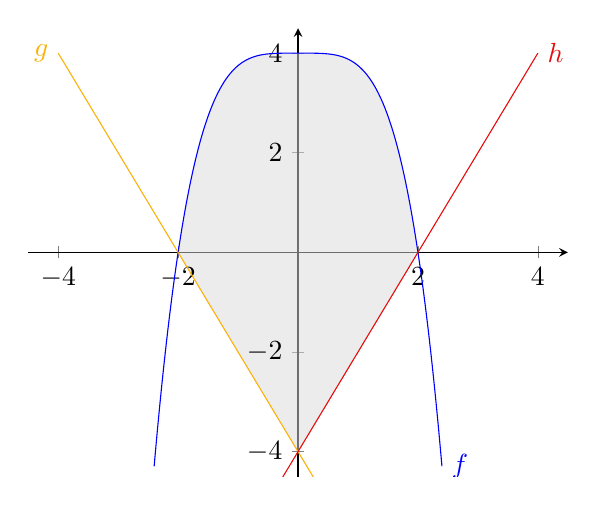
\begin{tikzpicture}
            \begin{axis}[
                    axis lines=middle,
                    xmin=-4.5,xmax=4.5,ymin=-4.5,ymax=4.5
                ]
                \addplot[blue, samples=1000, domain=-2.4:2.4, name path=A] {-0.25*x*x*x*x + 4} node[right] {$f$}; % f(x)
                \addplot[yellow!70!red, samples=300, domain=-4:4, name path=B] {-2*x - 4} node[pos=0, left] {$g$}; % g(x)
                \addplot[red!90!teal, samples=300, domain=-4:4, name path=C] {2*x-4} node[right] {$h$}; % h(x)
                \addplot[gray!30, opacity=0.5] fill between[of=A and C,soft clip={domain=0:2}];
                \addplot[gray!30, opacity=0.5] fill between[of=A and B,soft clip={domain=-2:0}];
            \end{axis}
        \end{tikzpicture}
    \end{center}

    Wir sehen in der Zeichnung, dass für die Fläche $A$ zwischen den Graphen gilt:
    $$
        \begin{aligned}
            A ={} & \abs{  \int_{-2}^{0} \left(f(x) - g(x)\right) \dx} + \abs{ \int_{0}^{2} \left(f(x) - h(x)\right) \dx}                           \\
            ={}   & \abs{ \int_{-2}^{0} \left(-\frac{1}{4}x^4 + 2x + 8\right) \dx} + \abs{ \int_{0}^{2} \left(-\frac{1}{4}x^4 - 2x + 8\right) \dx}  \\
            ={}   & \abs{ \left[ -\frac{1}{20}x^5 + x^2 + 8x \right]_{-2}^{0} } + \abs{ \left[ -\frac{1}{20}x^5 - x^2 + 8x \right]_0^2 }            \\
            ={}   & \abs{ 0 - \left( -\frac{1}{20}\cdot(-2)^5 + (-2)^2 + 8\cdot(-2) \right) } + \abs{ -\frac{1}{20}\cdot 2^5 + 2^2 + 8\cdot 2 - 0 } \\
            ={}   & \abs{-\frac{8}{5} - 4 + 16 } + \abs{-\frac{8}{5} - 4 + 16}                                                                      \\
            ={}   & \frac{52}{5} + \frac{52}{5}                                                                                                     \\
            ={}   & \frac{104}{5}
        \end{aligned}
    $$
    Damit beträgt der Flächeninhalt $\frac{104}{5}$ Flächeneinheiten. \qed
\end{bonus}

\newpage
\subsection{Längenberechnung}

\begin{algo}{Längenberechnung eines Graphen}
    Gegeben sind eine Funktion $f\in C[a, b]$ und die Punkte $a, b$.

    Die Länge $L_a^b$ des Graphen der Funktion $f$ ist dann gegeben mit
    $$
        L^b_a(f) = \int_a^b \sqrt{1+(f'(x))^2} \dx
    $$
\end{algo}

\subsection{Mantelflächenberechnung}

\begin{algo}{Mantelflächenberechnung}
    Gegeben sind eine Funktion $f\in C[a, b]$ und die Punkte $a, b$.

    Die Mantelfläche $M_a^b$ des Rotationskörpers der Funktion $f$ ist dann gegeben mit
    $$
        M^b_a(f) = \int_a^b 2\pi \cdot f(x) \cdot \sqrt{1+(f'(x))^2} \dx
    $$
\end{algo}

\subsection{Rotationsvolumenberechnung}

\begin{algo}{Rotationsvolumenberechnung}
    Gegeben sind eine Funktion $f\in C[a, b]$ und die Punkte $a, b$.

    Das Volumen $M_a^b$ des Rotationskörpers der Funktion $f$ ist dann gegeben mit
    $$
        V^b_a(f) = \int_a^b \pi \cdot f(x)^2 \dx
    $$
\end{algo}

\subsection{Differentiation von Integralen mit variablen Grenzen}

\begin{algo}{Differentiation von Integralen mit variablen Grenzen}
    Gegeben sei das Integral
    $$
        \int^{h(x)}_{g(x)} f(t)\dt.
    $$
    Dann gilt:
    $$
        \left(\int^{h(x)}_{g(x)} f(t)\dt\right)' = f(h(x)) \cdot h'(x) - f(g(x))\cdot g'(x).
    $$
\end{algo}

\subsection{Parameterintegrale}

\begin{defi}{Parameterintegral}
    Sei $f(x, t)$ eine von zwei rellen Parametern abhängige Funktion.
    Die Funktionen $g_1(x)$ und $g_2(x)$ seien stetig auf $[a, b]$ und differenzierbar auf $(a, b)$ sowie $f(x, t)$ integrierbar bez. $t$.

    Dann heißt
    $$
        F(x) = \int^{g_2(x)}_{g_1(x)} f(x, t) \dt
    $$
    das \emph{Parameterintegral}.
\end{defi}

\begin{example}{Parameterintegral}
    $$
        \begin{aligned}
            \lim_{x\to\infty} \left( \frac{1}{x} \cdot \int_0^x \frac{t+1}{t^2 + 2} \dt\right)
             & \overset{\text{de L'Hospital}}={} \lim_{x\to\infty} \left( \frac{1}{1} \cdot \left( \frac{x+1}{x^2 + 2} \cdot 1 - \frac{0+1}{0+2} \cdot 0 \right)\right) \\
             & ={} \lim_{x\to\infty} \left( \frac{x+1}{x^2 + 2} \right)                                                                                                 \\
             & ={} 0
        \end{aligned}
    $$\qed
\end{example}

\begin{defi}{Leibniz-Regel}
    Das Parameterintegral $F(x) = \int^{g_2(x)}_{g_1(x)} f(x, t) \dt$ ist differenzierbar und es ist
    $$
        F'(x) = f(x, g_2(x)) \cdot g'_2(x) - f(x, g_1(x)) \cdot g'_1(x) + \int^{g_2(x)}_{g_1(x)} \frac{\mathrm{d} f(x, t)}{\dx}\dt
    $$
\end{defi}

\begin{example}{Leibniz-Regel}
    $$F(x) = \int_{t=x}^{x^2} \frac{1}{t} \cdot \ln (1 + x\cdot t) \dt \quad (x>0)$$
    $$
        \begin{aligned}
            \dFdx
             & ={} \int_{t=x}^{x^2} \frac{1}{t} \cdot \ln (1 + x\cdot t) \dt                                                                                                                                \\
             & ={} \frac{1}{x^2} \cdot \ln (1 + x\cdot x^2) \cdot 2x - \left( \frac{1}{x} \cdot \ln (1 + x\cdot x) \cdot 1 \right) + \int^{x^2}_{t=x} \frac{1}{t} \cdot t \cdot \frac{1}{1 + x \cdot t} \dt \\
             & ={} \frac{2\ln (1 + x^3)}{x} - \frac{\ln(1+x^2)}{x} + \left[ \frac{\ln(1+x\cdot t)}{x} \right]^{x^2}_{t=x}                                                                                   \\
             & ={} \frac{2\ln (1 + x^3)}{x} - \frac{\ln(1+x^2)}{x} + \frac{\ln(1+x\cdot x^2)}{x} - \frac{\ln(1+x\cdot x)}{x}                                                                                \\
             & ={} \frac{3\ln (1 + x^3) - 2\ln(1+x^2)}{x}                                                                                                                                                   \\
        \end{aligned}
    $$\qed
\end{example}

\subsection{Uneigentliche Integrale}

\begin{defi}{Uneigentliche Integrale}
    Sei $f(x)$ beschränkt auf $\R$, dann definieren wir
    $$
        \begin{aligned}
            \int^\infty_a f(x) \dx         & := \lim_{R\to\infty} \int^R_a f(x)\dx                                          \\
            \int^b_{-\infty} f(x) \dx      & := \lim_{R\to\infty} \int^b_{-R} f(x)\dx                                       \\
            \int^\infty_{-\infty} f(x) \dx & := \lim_{R\to\infty} \int^R_{c} f(x)\dx + \lim_{R\to\infty} \int^c_{R} f(x)\dx
        \end{aligned}
    $$
\end{defi}

\begin{defi}{Konvergenz von Integralen}
    Die Integrale heißen \emph{konvergent}, wenn die Grenzwerte existieren, sonst heißen sie \emph{divergent}.
\end{defi}

\subsection{Absolute Konvergenz}

\begin{defi}{Absolute Konvergenz von Integralen}
    Sei $\int^b_a f(x) \dx$ ein eigentliches oder uneigentliches Integral.

    Konvergiert
    $$
        \int^b_a \abs{f(x)} \dx,
    $$
    so heißt $\int^b_a f(x) \dx$ \emph{absolut konvergent}.
\end{defi}

\subsection{Weitere Konvergenzkriterien}

\begin{defi}{Majoranten- und Minorantenkriterium für unbeschränkte Integrationsintervalle}
    Sei $\forall x \in [a, \infty) : 0 \leq \abs{f(x)} \leq g(x)$ und konvergiert $\int^\infty_a g(x)$, dann konvergiert $\int^\infty_a f(x) \dx$ und es gilt
    $$
        \abs{\int^\infty_a f(x) \dx} \leq \int^\infty_a \abs{f(x)} \dx \leq \int^\infty_a g(x) \dx.
    $$

    Ist $\forall x\in [a, \infty) : 0\leq g(x) \leq f(x)$ und divergiert $\int^\infty_a g(x) \dx$, so divergiert auch $\int^\infty_a f(x) \dx$.
\end{defi}

\begin{defi}{Majoranten- und Minorantenkriterium für unbeschränkte Integranden}
    Sei $\forall x \in [a, b] : 0 \leq \abs{f(x)} \leq g(x)$ und konvergiert $\int^b_a g(x)$, dann konvergiert $\int^b_a f(x) \dx$ und es gilt
    $$
        \abs{\int^\infty_a f(x) \dx} \leq \int^b_a \abs{f(x)} \dx \leq \int^b_a g(x) \dx.
    $$

    Ist $\forall x\in [a, b] : 0\leq g(x) \leq f(x)$ und divergiert $\int^b_a g(x) \dx$, so divergiert auch $\int^b_a f(x) \dx$.
\end{defi}

\subsection{Das Integralkriterium zur Konvergenz von Reihen}

\begin{defi}{Integralkriterium}
    Sei $f$ eine auf $[m-1, \infty]$ monoton fallende Funktion mit $\forall x \in [m, \infty) : f(x) \geq 0$, dann ist die Reihe
    $$
        \sum^\infty_{n=m} f(n)
    $$
    genau dann \emph{konvergent}, wenn
    $$
        \int^\infty_m f(x) \dx
    $$
    existiert. Es gilt bei Konvergenz
    $$
        \sum^\infty_{n=m+1} f(n) \leq \int^\infty_m f(x) \dx \leq \sum^\infty_{n=m} f(n) \leq \int^\infty_{m-1} f(x) \dx.
    $$
\end{defi}

\begin{example}{Integralkriterium}
    \[
        \sum^\infty_{n=1} \frac{1}{\sqrt[3]{n}} = \sum^\infty_{n=1} f(n)
    \]
    $f(n)$ ist offensichtlich auf dem Intervall $[1, \infty )$ streng monoton fallend.

    Damit muss nur geprüft werden, dass das Integral $\int^\infty_{n=1} f(n) \dn$ existiert bzw. konvergiert:

    $$
        \begin{aligned}
            \int^\infty_{n=1} f(n) \dn
             & ={} \int^\infty_{n=1} \frac{1}{\sqrt[3]{n}} \dn                              \\
             & ={} \lim_{b\to\infty} \left[ \frac{3n^{\frac{2}{3}}}{2} \right]^b_{n=1}      \\
             & ={} \lim_{b\to\infty} \left( \frac{3b^{\frac{2}{3}}}{2} - \frac{3}{2}\right) \\
             & ={} \infty
        \end{aligned}
    $$
    Damit divergiert das Integral und die gegebene Summe divergiert ebenfalls.\qed
\end{example}

\printindex
\printindex[Beispiele]
\end{document}
